\chapter{Feature Selection}
\section{Introduction}
Many algorithms, like the ones for classification or clustering, work with structured representations of texts. These representations, especially in the bag-ofwords form, suffer from many dimensions and sparsity. This generally decreases the performance of learning and the quality of achieved results [\cite{ref145}]. It is therefore desirable to lower the number of features because it is expected that some of the features are irrelevant (removing them does not affect learning) or redundant (correlated with another feature) [\cite{ref175}].

There are two possible approaches [\cite{ref179}, \cite{ref286}, \cite{ref159}, \cite{ref175}]:

\begin{itemize}
  \item Feature extraction - new features are derived from the data through some mapping of features to others. Methods based on the decomposition of a matrix representing the distribution of terms in documents, like the Latent Semantic Analysis, is one of the examples. A problem with these techniques might be bad interpretability of the newly created features.
  \item Feature selection - a subset from the original features is selected according to corpus statistics or some other criteria. The features can be ranked and the top $k$ or a minimal set that still enables satisfactory learning is selected.
\end{itemize}

In both approaches, it is desirable to select or extract the features automatically.

The main benefits of feature selection include [\cite{ref69}, \cite{ref201}, \cite{ref92}]:

\begin{itemize}
  \item Generalization of the model is better. This reduces overfitting and enables better learning accuracy.
  \item Efficiency of the algorithms increases. The time needed for computations, space for storing data, network bandwidth to transmit data can be decreased for the purpose of data collection, training, and execution.
  \item The crated model can be more easily understood, visualized (although it might not be possible to reduce the features to two or three dimensions so that the model can be examined by a human), and interpreted by a researcher.
\end{itemize}

Supervised feature selection methods rely on the knowledge of class labels of the data items. Then, the features that are somehow related to the labels are relevant. In an unsupervised problem, the class labels are missing, so feature selection is more complicated, but still desirable. The impact of feature selection needs to be evaluated differently. In a supervised selection, the features should be able to distinguish between the classes of data items, and common classification performance metrics, like accuracy, can be used. In unsupervised feature selection, the features should help reveal interesting groups in data. Clustering evaluation measure can be used here. The problem is that the number of clusters is usually not known in advance and also differs for different numbers of features (dimensions in the feature space) [\cite{ref78}].

The following approaches can generally be distinguished in feature selection. They can be used in supervised feature selection, as well as in unsupervised feature selection [\cite{ref47}, \cite{ref159}, \cite{ref137}, \cite{ref78}, \cite{ref119}]:

\begin{itemize}
  \item Wrapper approaches - a subset of features is evaluated by an algorithm (e.g., a classification algorithm) and by an evaluation metrics of that algorithm (e.g., classification accuracy). Because a new learner needs to be created for each subset, this approach might be very computationally demanding. On the other hand, this approach can lead to better performance as compared to a filter approach.
  \item Filter approaches - a subset of features is selected independently on an algorithm to be later applied to the data. It generally considers some discriminative ability of features, e.g., the ability to distinguish classes.
  \item Embedded approaches - a feature selection process is automatically embedded in an algorithm. An example is the selection of a feature for split in decision tree learning (e.g., the C4.5 algorithm [\cite{ref220}]) or W-k-means, a modified k -means algorithm which automatically determines important features [\cite{ref121}].
  \item Hybrid approaches - take advantage of both filter and wrapper approaches. An initial set of features is selected with computationally efficiat filters and then refined by more accurate wrappers.
\end{itemize}

\section{Feature Selection as State Space Search}
In order to find the best features for a given problem, all possible feature subsets should be examined. This is usually not feasible, so some search strategies are applied. To introduce some system to the process, a procedure systematically adding or removing features is usually applied. In other words, the state described by the features selected or unused for the given problem changes in a systematic manner. There are a certain number of possible states and transitions between them. The goal is to find a suitable path from an initial state to a state that satisfies given conditions (e.g., the features enable achieving small classification error). Several approaches to the definition of the states and transitions between them are in existence [\cite{ref27}]:

\begin{itemize}
  \item Forward selection - the feature set is empty at the beginning. The features are successively added until a suitable feature set is found. This can be seen as searching a state space where the states are described by selected and unused features; see Figure 14.1.
  \item Backward elimination - the feature set contains all features at the beginning. The features are successively eliminated as long as the features are useful. The states in the state space defined by selected and unused attributes are searched in the order inverse to the search in forward selection.
\end{itemize}

In order to visit all states during searching for a suitable feature set, $2^{m}$ possible states need to be visited ( $m$ is the number of features). In the text mining domain, where the data can be characterized by tens of thousands of features, this is sometimes not realistic. Instead of exhaustive state space search (which would guarantee finding an optimal feature set), some greedy approach that considers local changes between the states is applied. These heuristic approaches are, besides being less computationally demanding, often less prone to overfitting [\cite{ref175}].

The search strategies for traversing the state space include [\cite{ref137}, \cite{ref258}]:

\begin{itemize}
  \item Exponential methods - The number of feature subsets grows exponentially with the increasing feature space size. An example is the exhaustive search.
  \item Sequential methods - With the growing feature space size, only one or few subsets need to be evaluated. Greedy forward selection or backward elimination belong to this category.
  \item Randomized methods - Some of the steps in selecting features are randomized (for example, randomly selecting a subset of features). This usually increases the speed of computations and prevents trapping in a local optimum.
\end{itemize}

\begin{figure}[H]
\begin{center}
  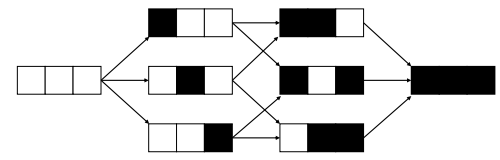
\includegraphics[width=0.8\textwidth]{chapter/chapter14/figure14_1.png}
\captionsetup{labelformat=empty}
\caption{\textbf{Figure 14.1:} Forward feature selection strategy. We start with en empty feature set and search the state space defined by the set of selected/unused features by adding additional features. At the end, all features are selected. If the arrows are inverted and we start with the full feature set, we talk about backward elimination.}
\label{fig14.1}
\end{center}
\end{figure}

\begin{figure}[H]
\begin{center}
  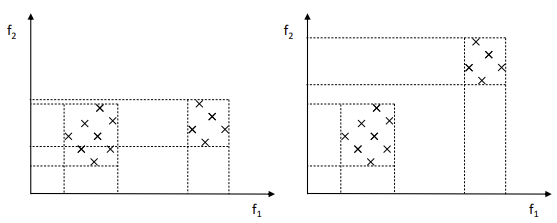
\includegraphics[width=0.8\textwidth]{chapter/chapter14/figure14_2.png}
\captionsetup{labelformat=empty}
\caption{\textbf{Figure 14.2:} Left: feature $f_{1}$ is able to separate the objects to two clusters. Feature $f_{2}$ is useless in this task, it is irrelevant. Right: both features can separate the objects to two clusters, but only one of them is enough. They contain redundant information [\cite{ref78}].}
\label{fig14.2}
\end{center}
\end{figure}

\section{Feature Selection Methods}
Wrapper methods often work better than filters because they are tailored to a specific problem. Their application is, however, often limited to smaller problems. On the other hand, filter methods are preferred for large scale problems, like text categorization, because of their lower computational costs [\cite{ref169}].

Commonly used filter approaches to feature selection in text mining include chi squared, mutual information, information gain, bi-normal separation (BNS) expected cross entropy, Gini index, odds ratio, term strength, entropy-based ranking, and term contribution [\cite{ref200}, \cite{ref137}, \cite{ref92}].

Supervised filter methods rank attributes according to their utility with respect to a given task (e.g., assigning a document to a class). This utility is assigned by a function that Li et al. [\cite{ref169}] call a score-computing function. Such functions, for a supervised task, usually work with probabilities that are esti-mated based on statistical information about distribution of terms in documents with different categories. These probabilities include:

\begin{itemize}
  \item $P\left(t_{i}\right)$ : the probability that a document contains term $t_{i}$
  \item $P\left(\bar{t}_{i}\right)$ : the probability that a document does not contain term $t_{i}$
  \item $P\left(c_{j}\right)$ : the probability that a document belongs to category $c_{j}$
  \item $P\left(\overline{c_{j}}\right)$ : the probability that a document does not belong to category $c_{j}$
  \item $P\left(t_{i}, c_{j}\right)$ : the joint probability that a document contains term $t_{i}$ and also belongs to category $c_{j}$
  \item $P\left(c_{j} \mid t_{i}\right)$ : the probability that a document belongs to category $c_{j}$ given that it contains term $t_{i}$
  \item $P\left(c_{j} \mid \bar{t}_{i}\right)$ : the probability that a document belongs to category $c_{j}$ given that it does not contain term $t_{i}$
  \item $P\left(\bar{c}_{j} \mid t_{i}\right)$ : the probability that a document does not belong to category $c_{j}$ given that it contains term $t_{i}$
  \item $P\left(t_{i} \mid c_{j}\right)$ : the probability that a document contains term $t_{i}$ given that it belongs to category $c_{j}$
  \item $P\left(t_{i} \mid \overline{c_{j}}\right)$ : the probability that a document contains term $t_{i}$ given that it does not belong to category $c_{j}$
  \item $P\left(\bar{t}_{i} \mid c_{j}\right)$ : the probability that a document does not contain term $t_{i}$ given that it belongs to category $c_{j}$
\end{itemize}

These probabilities can be only estimated with some statistical information from the training data:

\begin{itemize}
  \item $A_{j}$ : the number of documents that contain term $t_{i}$ and also belong to category $c_{j}$
  \item $B_{j}$ : the number of documents that contain term $t_{i}$ but do not belong to category $c_{j}$
  \item $\quad N_{j}$ : the number of documents that belong to category $c_{j}$
  \item $N$ : the total number of documents
  \item $C_{j}$ : the number of documents that do not contain term $t_{i}$ but belong to category $c_{j}$; can be calculated as $N_{j}-A_{j}$
  \item $D_{j}$ : the number of documents that neither contain term $t_{i}$ nor belong to category $c_{j}$; can be calculated as $N-N_{j}-B_{j}$
\end{itemize}

For unsupervised methods, no information is available about class. The suitability of a feature with respect to a given task can thus be derived only from the data itself. Unsupervised methods, like term contribution, are sometimes criticized because they rely on a particular similarity function (typically the cosine similarity); see below. When a different similarity function would be used, different terms might be selected as relevant [\cite{ref7}]. When many computations need to be performed, e.g., when calculating the similarity of all document pairs, sampling can be used in real experiments [\cite{ref179}].

\subsection{\texorpdfstring{Chi Squared ( $\chi^{2}$ )}{Chi Squared (Chi-2)}}
The Chi-squared test is used in statistics to measure independence of two events measured by two categorical variables. To test this independence, a random sample is selected, the properties of these objects are studied, and a contingency table with frequencies is created. We might, for example, study whether gender and selected majors in a university are related. Randomly picked 100 men and 100 women are asked to tell their major and the frequencies of specific gendermajor pairs are counted (e.g., 20 men study Computer Science). The gender and major variables are then tested for their independence [\cite{ref264}].

The test measures how what is observed is different from what is expected. If, for example, you toss a fair coin ten times, you expect that it will land five times on tails and five times on heads (tossing a coin eleven times, one would expect 5.5 tails and 5.5 heads, which, of course, is not realistic) [\cite{ref251}].

The null hypothesis, which is tested, is that there is no statistically significant difference between the expected and observed frequencies [\cite{ref132}]. To get the expected frequencies, row and column marginals are multiplied and then divided by the sum of all cells in the contingency table. Then, the $\chi^{2}$ value is calculated as the sum of the squares of differences between the observed and expected values divided by the expected values [\cite{ref93}]:


\begin{equation*}
\chi^{2}=\sum \frac{(O-E)^{2}}{E}, \tag{14.1}
\end{equation*}


where $O$ is the observed frequency and $E$ is the expected frequency. The calculated value of $\chi^{2}$ is compared to the critical $\chi^{2}$ value (usually the 95 th percentile of the $\chi^{2}$ distribution with one degree of freedom) to see how significant the difference between the observed and expected frequencies is [\cite{ref48}].

The Chi-squared score can be used to measure the dependence between a term and category. The occurrences of the term and the class, both having values yes or no are the two events studied. The value of $\chi^{2}$ can be calculated as follows [\cite{ref185}]:


\begin{equation*}
\chi^{2}(t, c)=\sum_{e_{t} \in\{\text { yes,no }\}} \sum_{e_{c} \in\{\text { yes,no }\}} \frac{\left(O_{e_{t} e_{c}}-E_{e_{t} e_{c}}\right)^{2}}{E_{e_{t} e_{c}}}, \tag{14.2}
\end{equation*}


where $O$ is the observed frequency, $E$ is the expected frequency, and $e_{x}$ is the number of documents containing or not containing term $t$ and belonging or not belonging to class $c$ (for example, $e_{t}=y e s, e_{c}=y e s$ is the number of documents containing term $t$ and belonging to class $c$ ).

Considering the statistics defined above, the value of $\chi^{2}$ can be calculated as follows [\cite{ref286}]:


\begin{equation*}
\chi(t, c)=\frac{N\left(A_{j} D_{j}-C_{j} B_{j}\right)^{2}}{\left(A_{j}+C_{j}\right)\left(B_{j}+D_{j}\right)\left(A_{j}+B_{j}\right)\left(C_{j}+D_{j}\right)} \tag{14.3}
\end{equation*}


If the term and category are independent, the value of $\chi^{2}$ is equal to zero. Higher values mean that some dependency exists between the class and the term. In other words, the occurrence of a term makes a class more or less likely.

To calculate the overall usefulness of a term (not just for one specific class), a weighted average over all classes is calculated [\cite{ref82}]:


\begin{equation*}
\chi(t)=\sum_{j=1}^{k} P\left(c_{j}\right) \chi^{2}\left(t, c_{j}\right), \tag{14.4}
\end{equation*}


where $P\left(c_{j}\right)$ is the probability of category $c_{j}$.\\
In text categorization, no statements about statistical independence need to be made and absolute values of $\chi^{2}(t, c)$ are not that important. Instead, the relative importance of features is interesting and the values of $\chi^{2}(t, c)$ are used to rank the terms. Useful terms that are able to distinguish classes have high values of $\chi^{2}(t, c)$ [\cite{ref185}]. The values of $\chi^{2}$ are normalized so they can be used to compare terms in one category. However, this normalization is broken when there are low frequency terms [\cite{ref286}].

\subsection{Mutual Information}
In the information theory, information is contained in a sequence of messages that are transmitted from a source to a receiver; it is expected to be useful in reducing uncertainty about an event. The content of the messages can be studied and quantified in terms of the element of uncertainty or surprise they bring. If we have a source sending only one possible message, we are pretty sure about its content. In other words, we are not surprised at all after seeing the message. If there are two equally possible outcomes, the chance of receiving one of them is $50 \%$. One of 10 possible messages, equally likely to occur, the probability of receiving one of them will be $10 \%$. We can see that with the growing number of possible outcomes, our uncertainty about the incoming message generally increases. The surprise is also related to the probability with which the different messages occur. Having two possible outcomes X and Y where X will be more likely to occur than Y , we will be more certain about the incoming message because we will see $X$ more often.

To be able to measure uncertainty (surprise) of the outcome of a message, Shannon [249] defined information of a message, $x$, that comes from a set of all possible messages $X$ as:


\begin{equation*}
I(x)=\log \frac{1}{p(x)}=-\log p(x) \tag{14.5}
\end{equation*}


where $p(x)$ is the probability of message $x$. The base of the logarithm is often 2 because many things are boolean in nature. Messages are also often encoded using zeros and ones in computer memories. The unit of information is then known as a bit or shannon. When there are just two possible messages, like when tossing a fair coin, the information of a head will be $-\log _{2} 0.5=1$ bit. Having hexadecimal digits, the information associated with each of them equals to $-\log _{2} 1 / 16=4$ bits.

The amount of information is related to the size of a message, e.g., in a communication channel. The value of $\frac{1}{p(x)}$ in the formula is actually the number of choices when the probabilities of each message are equal. To encode a coin toss, outcome, one binary digit is needed. To encode a hexadecimal digit, four binary digits are necessary. But what if we have a fair die? Then, each number on it will carry information $-\log _{2} 1 / 6=2.58$ bits. It means that 2.58 binary digits are needed to encode a message. How we can use only a part of a binary digit? A better option is to think about asking questions allowing either yes or no answers that will subsequently divide all possible answers into two equally sized halves. Let us look at the example of guessing a number between 1 and 8 where, for instance, 7 is the right answer. The following questions might be asked:

\begin{itemize}
  \item Is the number less or equal to 4 ? No - the number must be $5,6,7$, or 8 .
  \item Is the number greater or equal to 7 ? Yes - the number must be 7 or 8 .
  \item Is the number 8 ? No - the number must be 7 .
\end{itemize}

We asked three questions to receive the correct answer, which equals to $-\log 1 / 8$. The more the questions which need to be asked, the more the information a message contains. We can look at the measure (of uncertainty) as the amount of missing information that is required to specify an outcome [\cite{ref164}]. If the amount of information is not an integer number, we can treat is as the average number of questions to be asked to get a correct answer.

When some of the answers are more likely, it is better to ask questions so that their number is minimized (i.e., ask for the most likely answer). When relating this to encoding messages, it is better to encode more likely answers using a lower number of symbols (bits) because they will occupy less space. A well known example is the Morse code where more frequent letters, like $\mathrm{E}, \mathrm{T}, \mathrm{A}$, or I have less symbols than, for example, $\mathrm{Z}, \mathrm{H}$, or Q . The Morse code is, however, not a good application for computers because it requires three symbols (dot, dash, space).

To encode letters of the English alphabet (26 symbols in total), $-\log _{2} 1 / 26=$ 4.7 bits, which means 5 bits of a fixed code would be needed. When considering the different frequency of the letters and, for example, a Huffman code, only 4.13 bits are needed on average (the most frequent letter, E , will be encoded as 000 , A will become 0011, and the least frequent letter, Z , will be 1111111) [\cite{ref266}, \cite{ref233}].

A measure of the average amount of information of a message with $n$ possibilities, when the probabilities $p_{1}, p_{2}, \ldots, p_{n}$ are taken into consideration, is known as entropy. Shannon [\cite{ref249}] found a function $H\left(p_{1}, p_{2}, \ldots, p_{n}\right)$ that was the only one satisfying several important properties: is continuous in its parameters, is a monotonic increasing function of $n$ when $p_{1}=p_{2}=\ldots p_{n}=\frac{1}{n}$, and is the weighted sum of the individual values of $H$ when a choice is broken down into two successive choices.

The formula for calculating entropy, which is actually the weighted average of entropies of individual outcomes (weighted by their probability), is:


\begin{equation*}
H=\sum_{i=1}^{n} p_{i} \log p_{i} \tag{14.6}
\end{equation*}


The logarithmic measure expressing the information of one message selected from several possible messages where all choices are equally likely, is the most natural choice because many important parameters in engineering vary linearly with the logarithm of the number of possibilities. When there are $N$ events with two possible outcomes, adding another such event will double the number of possible outcome combinations. This is expressed by the increase by 1 of the base 2 logarithm of the number of possible outcomes.

When there is only one possible outcome of an event, the value of entropy for this information is $H=-1 \log 1=0$. If the source sends two possible messages with the same probability (like, e.g., in the case of tossing a fair coin), the surprise can be quantified by entropy $h=-\left(0.5 \log _{2} 0.5+0.5 \log _{2} 0.5\right)=1$ bit. Having two possible outcomes where one has a higher probability, say $70 \%$ (for example, an unfair coin flipping), the entropy will be $H=-\left(0.7 \log _{2} 0.7+0.3 \log _{2} 0.3\right)=$ 0.88 bits. When there are more than two outcomes, for example, when rolling a fair die, the entropy will have the value $H=-6\left(1 / 6 \log _{2} 1 / 6\right)=2.58$ bits. We can see that entropy (our surprise) is higher when there are more possible outcomes and when the outcomes have equal probability.

When there are two random variables $x$ and $y$, the Pointwise Mutual Information (PMI) can be calculated for two outcomes $x \in X$ and $y \in Y$ as follows [\cite{ref85}]:


\begin{equation*}
P M I(x, y)=\log \frac{p(x \mid y)}{p(x)}=\log \frac{p(x, y)}{p(x) p(y)}=\log \frac{p(y \mid x)}{p(y} \tag{14.7}
\end{equation*}


Taking logarithm out of consideration, the formulae calculate the ratio of the probability when $x$ and $y$ co-occur and when they were independent. The logarithm is used to measure this value in bits (when the base is 2 ). It can be\\
interpreted as the amount of information provided by the occurrence of $x$ about the occurrence of $y$ [\cite{ref85}]. The value of PMI equals zero when the events $x$ and $y$ are independent, i.e., $p(x, y)=p(x) p(y)$. When there is an association between $x$ and $y$, the probability $p(x, y)$ will be greater than $p(x) p(y)$ and thus PMI $>0$. If one event occurs while the other tends not to, which is known as complementary distribution, the value of PMI is negative [\cite{ref25},\cite{ref52}].

When considering all possible outcomes of two random variables $X$ and $Y$, mutual information is the average pointwise mutual information for all possible pairs $x \in X$ and $y \in Y$. It is, again, a weighted average where the weights are the probabilities that $x$ and $y$ co-occur:


\begin{equation*}
I(X, Y)=\sum_{x \in X} \sum_{y \in Y} p(x, y) \log \frac{p(x, y)}{p(x) p(y)} \tag{14.8}
\end{equation*}


Mutual information measures how much information about one variable is contained in another variable.

When measuring joint entropy of two variables $X$ and $Y$ (uncertainty associated to co-occurrence of values of two variables), we measure average information for all possible outcomes $x \in X$ and $y \in Y$ :


\begin{equation*}
H(X, Y)=-\sum_{x \in X} \sum_{y \in Y} p(x, y) \log p(x, y) \tag{14.9}
\end{equation*}


The joint entropy $H(X, Y)$ is always non-negative, greater than or equal to $H(X)$ or $H(Y)$, and less than or equal to the sum of individual entropies:


\begin{gather*}
H(X, Y) \geq 0 \\
H(X, Y) \geq \max [H(X), H(Y)]  \tag{14.10}\\
H(X, Y) \leq H(X)+H(Y)
\end{gather*}


If the variables $X$ and $Y$ are independent, the information contained in their combination equals the sum of individual entropies. If the variables are somehow dependent, they provide less information in their combination. This smaller amount information is quantified by their mutual information:


\begin{equation*}
I(X, Y)=H(X)+H(Y)-H(X, Y) \tag{14.11}
\end{equation*}


The joint entropy can also be related to the conditional entropy. The conditional entropy measures how much information is contained in one variable when the other is known. When we know the value of variable $X$, the conditional entropy $H(Y \mid X=x)$ can be calculated as follows:


\begin{equation*}
H(Y \mid X=x)=-\sum_{y \in Y} p(y \mid x) \log p(y \mid x) \tag{14.12}
\end{equation*}


The conditional entropy $H(Y \mid X)$ is then an average of $H(Y \mid X=x)$ for all possible values of $x$ :


\begin{align*}
H(Y \mid X) & =\sum_{x \in X} p(x) H(Y \mid X=x) \\
& =-\sum_{x \in X} p(x) \sum_{y \in Y} p(y \mid x) \log p(y \mid x)  \tag{14.13}\\
& =-\sum_{x \in X} \sum_{y \in Y} p(x, y) \log p(y \mid x)
\end{align*}


Mutual information can also be interpreted as the information contained in one variable minus the information contained in the variable when the other variable is known [104]:


\begin{equation*}
I(X, Y)=H(Y)-H(Y \mid X)=H(X)-H(X \mid Y) \tag{14.14}
\end{equation*}


Mutual information can be used to measure how a class $c \in C$ and term $t \in V$ occur together, in other words, how much information about the classes the terms carry. An ideal situation would be achieved when a subset $s \subset V$ has the same mutual information with $C$ as $V$ has with $C$ :


\begin{equation*}
I(S, C)=I(V, C) \tag{14.15}
\end{equation*}


Because this problem is intractable, features with high mutual information with $C$ are included in $S$ so $I(S, C)$ is close to $I(V, C)$ [\cite{ref176}].

To evaluate how a term $t$ and class $c$ are correlated, their mutual information can be estimated as follows:


\begin{equation*}
I(t, c)=\log \frac{A N}{(A+C)(A+B)} \tag{14.16}
\end{equation*}


In order to measure the contribution of a term in assigning a class globally, there are a few ways in which the term-category scores can be combined into one score [\cite{ref286}]:


\begin{equation*}
I_{\text {avg }}(t)=\sum_{i=1}^{m} p\left(c_{i}\right) I\left(t, c_{i}\right) I_{\text {max }}(t)=\max i=1^{m}\left[I\left(t, c_{i}\right)\right] \tag{14.17}
\end{equation*}


A weakness of the mutual information measure is that it assigns higher scores to rare terms that have the same conditional probability $p(t \mid c)$ as common terms [\cite{ref286}].

\subsection{Information Gain}
Values of some features are related to specific classes and it is expected that instances from different classes will have different values of these features. For\\
example, body height is expected to be higher for adults and lower for children. If such a relationship is ideal, after partitioning all instances to be classified according to the value of a specific feature, we will have groups where there are instances of only one class in each group (e.g., in a group where body height is high there will only be adults, in the other group where body height is low only children will be present). We can say, that after partitioning one heterogeneous group of instances (with several mixed classes), we get several sets of homogeneous data (with only one class in a group).

The concept of entropy can be used to quantify how well a feature contributes to such partitioning. Entropy is used to measure the surprise of seeing an instance of a specific class in a set. The original heterogeneous set contains instances of several classes and the data is thus characterized by a certain level of entropy which is rather high. After having several more homogeneous sets where instances of one class prevail, the level of entropy will be lower. The feature thus contributes to the elimination of entropy that measures a disorder in the data.

Reduction of entropy (uncertainty) is related to information which needs to be sent to describe the data. When the data is heterogeneous, more information is needed than when there are several homogeneous sets. We thus gain some information that does not need to be sent. The measure quantifying such a contribution of an attribute is known as information gain.

The value of information gain for term $t_{i}$ can be calculated as the difference between the entropy of the set containing all data and the average entropy of sets that are the result of splitting the data according to the values of attribute $t_{i}$ [\cite{ref199}]:


\begin{equation*}
I G\left(t_{i}\right)=\operatorname{Entropy}(S)-\sum_{v \in \text { values }\left(t_{i}\right)} \frac{\left|S_{v}\right|}{|S|} \operatorname{Entropy}\left(S_{v}\right), \tag{14.18}
\end{equation*}


where $S$ is the set containing all data, values $\left(t_{i}\right)$ is a set of all possible values of feature $t_{i}$, and $S_{v}$ is a subset of $S$ where the value of $t_{i}$ is $v$. The entropy of data after partitioning is calculated as the weighted average of individual entropies where the weights are the relative sizes of the sets.

When we consider only presence or absence of a feature (i.e., presence or absence of a word in a text) information gain can be calculated as


\begin{align*}
I G\left(t_{i}\right)= & -\sum_{j=1}^{m} p\left(c_{j}\right) \log p\left(c_{j}\right) \\
& +p\left(t_{i}\right) \sum_{j=1}^{m} p\left(c_{j} \mid t_{i}\right) \log p\left(c_{j} \mid t_{i}\right)  \tag{14.19}\\
& +p\left(\overline{t_{i}}\right) \sum_{j=1}^{m} p\left(c_{j} \mid \overline{t_{i}}\right) \log p\left(c_{j} \mid \overline{t_{i}}\right)
\end{align*}


where $m$ is the number of classes, and $p\left(t_{i}\right)$ and $p\left(\bar{t}_{i}\right)$ are the probabilities that term $t_{i}$ appears or does not appear in a document.

The value of information gain can be estimated as follows [\cite{ref169}]:


\begin{align*}
I G\left(t_{i}\right)= & -\sum_{j=1}^{m} \frac{N_{j}}{N_{\text {all }}} \log \frac{N_{j}}{N_{\text {all }}} \\
& +\sum_{j=1}^{m} \frac{A_{j}}{N_{\text {all }}} \sum_{j=1}^{m} \frac{A_{j}}{A_{j}+B_{j}} \log \frac{A_{j}}{A_{j}+B_{j}}  \tag{14.20}\\
& +\sum_{j=1}^{m} \frac{C_{j}}{N_{\text {all }}} \sum_{j=1}^{m} \frac{C_{j}}{C_{j}+D_{j}} \log \frac{C_{j}}{C_{j}+D_{j}}
\end{align*}


Information gain is an important metric for determining the suitability of algorithms in the induction of decision trees with the 4.5 algorithm; see [\cite{ref7}]. The method is actually embedded in the algorithm.

\section{Term Elimination Based on Frequency}
Frequency based approaches to feature selection do not usually perform as well as other, more sophisticated methods, but often bring acceptable results [\cite{ref175}]. They are based on a simple idea that the frequency with which a term appears is related to its importance.

Terms appearing too frequently usually do not have a discriminative ability. Words like the, in, or have are contained in almost every document and are not specific for one class of documents. They are also not able to clearly characterize a group of documents in a clustering problem for the same reason. The common terms are known as stop words. Many lists of commonly used stop words are available in many languages. They usually contain about $300-400$ terms [\cite{ref7}].

Rare terms, on the other hand, can distinguish classes in classification. If a term appears in only one document from a specific class, one can think about using it when deciding on a class label. However, the goal of a learning algorithm is to find a generalization of class label assignment. A decision based on only one evidence would not be very general and will most likely lead to overfitting. Rare terms do not contribute significantly to calculating similarity in either. These rare terms are often noise in the data and represent mistyping or other language errors.

The rare and common terms can be easily eliminated without significant impact on the performance of a learner in a classification or clustering problem [\cite{ref270}, \cite{ref64}]. In an information retrieval task, rare terms are considered to be informative. Thus, strong reduction of these terms is not recommended [\cite{ref286}].

The frequencies used to determine a term's importance can be document frequencies or the total frequencies. Document frequency is more suitable for the

Bernoulli model (when the presence or absence of a term in a document is important), the total frequency is better for the multinomial model (when we have information about the frequency of a term in a document) [\cite{ref185}].

Another possibility is to work only with terms that are most common in a class. Of course, many stop words bringing no specific information of the class will be included but when a sufficient number of features is used, the results are acceptable [\cite{ref185}].

\section{Term Strength}
The Term Strength measure was originally proposed by Wilbur and Sirotkin [\cite{ref278}] to automatically discover stop words in information retrieval. The term strength, or importance, is based on the occurrence of a term in related documents. If the labels of documents are known, related documents belong to the same category. If the labels are unknown, the relatedness can be defined by a human. This is, however, often impractical so the relatedness is calculated using a document similarity, typically the Cosine similarity (it is expected that related documents share some words and the similarity is high). It is necessary to define a minimum threshold level for the similarity in order to consider two documents be related.

The term strength measures the probability with which a term occurs in the second document in a highly related pair of documents, knowing that it also occurs in the first one:


\begin{equation*}
s(w)=p\left(w \in d_{j} \mid w \in d_{i}\right), d_{i} \neq d_{j} \tag{14.21}
\end{equation*}


To estimate the term strength, we can randomly pick pairs of documents from the entire collection and calculate:


\begin{equation*}
s(w)=\frac{\text { number of pairs where } w \text { occurs in } d_{i} \text { and } d_{j}}{\text { number of pairs where } w \text { occurs in } d_{i}} \tag{14.22}
\end{equation*}


A term is expected to be a stop word (thus, an irrelevant word) if its term strength significantly differs from the term strength of a random term (a term randomly distributed in training documents with the same frequency). The significant difference means that the actual term strength is less than or equal to the term strength of a random word (expected term strength) plus twice the standard deviation of this term strength [\cite{ref7}]. To see the details regarding the calculation of the expected term strength of a random term and its random deviation, see [\cite{ref278}].


\section{Term Contribution}
Term Contribution was proposed by Liu et al. [\cite{ref179}] for selecting relevant terms for clustering. In clustering, similarity of documents is of great importance, so Term Contribution measures how a term contributes to document similarity. When calculating the similarity, the cosine similarity is considered as the similarity measure. The similarity of two documents, $d_{i}$ and $d_{j}$, is calculated as the dot product of the length normalized feature vectors representing the documents:


\begin{equation*}
\operatorname{sim}\left(d_{i}, d_{j}\right)=\sum_{t} w\left(t, d_{i}\right) \times w\left(t, d_{j}\right), \tag{14.23}
\end{equation*}


where $w$ represents a normalized tf-idf weight of term $t$ in document $d_{i}$ or $d_{j}$. In a $d_{i}$ or $d_{j}$ document pair, term $t_{t}$ contributes to the dot product (i.e., the similarity) with $w\left(t_{t}, d_{i}\right) \times w\left(t_{t}, d_{j}\right)$. Term contribution of the term is calculated as the sum of these contributions over all pairs in the document collection $D$ :


\begin{equation*}
T C\left(t_{t}\right)=\sum_{d_{i}, d_{j} \in D, d_{i} \neq d_{j}} w\left(t, d_{i}\right) \times w\left(t, d_{j}\right) \tag{14.24}
\end{equation*}


Terms with high scores of Term Contribution are considered to be relevant.

\section{Entropy-Based Ranking}
This measure is based on distinguishing between data with and without clusters. When clusters exist, objects in a cluster are expected to be close to each other in a feature space. Some of the features contribute to partitioning objects into clusters more than others and are thus important. Their usefulness is based on the idea that, after removing them, clustering will not be that obvious.

The distribution of objects in a feature space, in other words a disorder in the space, can be measured by entropy. If the probability of each point is equal, in other words, the objects are uniformly distributed, entropy is maximal.

To estimate the entropy (normalized to the interval $[0,1]$ ) of a collection of $n$ documents, similarities $S_{i j}$ between all pairs of objects $X_{i}$ and $X_{j}$ are used in calculations [63]:


\begin{equation*}
E=-\sum_{i=1}^{n} \sum_{j=1}^{n}\left[S_{i j} \log S_{i j}+\left(1-D_{i j}\right) \log \left(1-D_{i j}\right]\right. \tag{14.25}
\end{equation*}


The quality of a term is calculated as an entropy reduction when a term is removed from the collection [\cite{ref7}].

\section{Term Variance}
The Term Variance measure proposed by Liu et al. [\cite{ref178}] is based on the simple idea that important terms have high document frequencies and are not distributed uniformly. That means that they appear with higher frequencies in some documents and with lower frequencies in other documents. Terms appearing in just a few documents or having low variance will have a low Term Variance value. Term Variance of term $w_{i}$ in a collection of $n$ documents can be calculated as follows:


\begin{equation*}
T V\left(w_{i}\right)=\sum_{j=1}^{n}\left(f_{i j}-\bar{f}_{i}\right)^{2}, \tag{14.26}
\end{equation*}


where $f_{i j}$ is the frequency of term $w_{i}$ in $j^{\text {th }}$ document and $\bar{f}_{i}$ is the average frequency of $w_{i}$ in documents.

\section{An Example}
In the example, consider that we have 30 documents in three categories (sport, politics, and technology). We look only at a few terms (today, and, football, hockey, poll, minister, meeting, computer, and learning) and their presence in the documents in the three classes. A document-term matrix, together with document class labels representing the newspaper articles, can be found in Figure 14.9.

A summary containing the distribution of terms in the three categories is in Figure 14.4. We can see that the words are distributed differently in individual classes. Some of them, like the word today, appear with almost the same frequency in all classes; others, like hockey or learning, seem to be more specific for only some categories.\\[0.1cm]
To quantify the importance of terms in the task of assigning a class label, the values of some feature selection metrics can be calculated.\\[0.1cm]
Some already implemented feature selection algorithms are contained, for example, in package FSelector. The package provides algorithms for filtering attributes (e.g., functions chi.squared(), information.gain()), for wrapping classifiers and searching the attribute subset space using backward and forward search, and for choosing a subset of attributes.\\[0.1cm]
In the example, a document-term matrix is created and passed to one method (information gain) of feature selection from package FSelector. Several functions of the package are used to show the most important features and to remove the unimportant features from the data.

\begin{table}[H]
\begin{center}
\begin{tabular}{|c|c|c|c|c|c|c|c|c|l|}
\hline
% Rotated headers
\rotatebox{90}{today} & 
\rotatebox{90}{and} & 
\rotatebox{90}{football} & 
\rotatebox{90}{hockey} & 
\rotatebox{90}{poll} & 
\rotatebox{90}{minister} & 
\rotatebox{90}{meeting} & 
\rotatebox{90}{computer} & 
\rotatebox{90}{learning} & 
CLASS \\
\hline
% Data rows
0 & 0 & 1 & 0 & 0 & 0 & 0 & 0 & 0 & sport \\
1 & 0 & 1 & 1 & 0 & 0 & 0 & 0 & 0 & sport \\
0 & 1 & 0 & 0 & 0 & 1 & 0 & 1 & 0 & sport \\
0 & 0 & 0 & 1 & 0 & 0 & 0 & 0 & 1 & sport \\
1 & 0 & 1 & 0 & 1 & 0 & 1 & 0 & 0 & sport \\
1 & 1 & 1 & 0 & 0 & 0 & 1 & 0 & 0 & sport \\
0 & 0 & 1 & 1 & 0 & 0 & 0 & 0 & 1 & sport \\
1 & 0 & 0 & 1 & 0 & 0 & 0 & 0 & 0 & sport \\
0 & 1 & 1 & 0 & 0 & 1 & 0 & 1 & 0 & sport \\
0 & 0 & 1 & 0 & 0 & 0 & 1 & 0 & 0 & politics \\
1 & 1 & 0 & 0 & 1 & 1 & 0 & 0 & 0 & politics \\
0 & 0 & 0 & 0 & 0 & 1 & 0 & 0 & 1 & politics \\
0 & 1 & 0 & 0 & 0 & 0 & 1 & 0 & 0 & politics \\
1 & 1 & 0 & 1 & 0 & 0 & 0 & 0 & 0 & politics \\
1 & 1 & 0 & 0 & 1 & 0 & 0 & 0 & 0 & politics \\
1 & 0 & 1 & 0 & 0 & 1 & 1 & 0 & 1 & politics \\
0 & 1 & 0 & 0 & 1 & 0 & 0 & 1 & 0 & politics \\
1 & 0 & 0 & 0 & 0 & 1 & 0 & 0 & 0 & politics \\
1 & 1 & 0 & 0 & 1 & 0 & 1 & 0 & 0 & politics \\
1 & 0 & 1 & 0 & 0 & 0 & 0 & 0 & 1 & technology \\
0 & 1 & 1 & 0 & 0 & 0 & 0 & 0 & 1 & technology \\
1 & 1 & 0 & 1 & 0 & 0 & 1 & 0 & 0 & technology \\
0 & 1 & 0 & 0 & 0 & 1 & 0 & 1 & 0 & technology \\
1 & 0 & 1 & 0 & 0 & 0 & 0 & 0 & 1 & technology \\
1 & 0 & 0 & 0 & 0 & 0 & 0 & 0 & 0 & technology \\
1 & 1 & 0 & 0 & 0 & 1 & 0 & 1 & 1 & technology \\
1 & 1 & 0 & 0 & 1 & 0 & 1 & 0 & 0 & technology \\
0 & 1 & 0 & 1 & 0 & 0 & 0 & 0 & 1 & technology \\
0 & 0 & 0 & 0 & 0 & 0 & 0 & 1 & 0 & technology \\
\hline
\end{tabular}
\captionsetup{labelformat=empty}
\caption{\textbf{Figure 14.3:} A term document matrix representing the distribution of nine terms in thirty documents from three classes. The matrix also contains class labels.}
\label{fig14.3}
\end{center}
\end{table}

The values of another method (Chi squared) are calculated using coefficients $\mathrm{A}, \mathrm{B}, \mathrm{C}$, and D , introduced earlier in this chapter. The most important features characterizing the classes are also presented. The features that have high values of Chi squared are shown here. A feature does not have to be present in documents from a class in order to have a high value (if it is not there, it also demonstrates some correlation between the feature and class). Thus, only features that appear in the classes with higher than average frequency are displayed.

\begin{table}[H]
\begin{center}
\begin{tabular}{l|ccc}
\hline
 & \rotatebox{90}{sport} & \rotatebox{90}{politics} & \rotatebox{90}{technology} \\
\hline
today    & 5 & 6 & 6 \\
and      & 4 & 6 & 6 \\
football & 6 & 2 & 3 \\
hockey   & 5 & 1 & 2 \\
poll     & 1 & 4 & 1 \\
minister & 2 & 4 & 2 \\
meeting  & 3 & 4 & 2 \\
computer & 2 & 1 & 3 \\
learning & 2 & 2 & 5 \\
\hline
\end{tabular}
\captionsetup{labelformat=empty}
\caption{\textbf{Figure 14.4:} Frequencies of terms across three categories of newspaper articles.}
\label{fig14.4}
\end{center}
\end{table}

\begin{verbatim}
# a vector to be converted to a matrix representing
# the distribution of terms in documents
d <- c(
    1,1,0,1,0,0,1,0,0,
    0,0,1,0,0,0,0,0,0,
    1,0,1,1,0,0,0,0,0,
    0,1,0,0,0,1,0,1,0,
    0,0,0,1,0,0,0,0,1,
    1,0,1,0,1,0,1,0,0,
    1,1,1,0,0,0,1,0,0,
    0,0,1,1,0,0,0,0,1,
    1,0,0,1,0,0,0,0,0,
    0,1,1,0,0,1,0,1,0,
    0,0,1,0,0,0,1,0,0,
    1,1,0,0,1,1,0,0,0,
    0,0,0,0,0,1,0,0,1,
    0,1,0,0,0,0,1,0,0,
    1,1,0,1,0,0,0,0,0,
    1,1,0,0,1,0,0,0,0,
    1,0,1,0,0,1,1,0,1,
    0,1,0,0,1,0,0,1,0,
    1,0,0,0,0,1,0,0,0,
    1,1,0,0,1,0,1,0,0,
    1,0,1,0,0,0,0,0,1,
    0,1,1,0,0,0,0,0,1,
    1,1,0,1,0,0,1,0,0,
    0,1,0,0,0,1,0,1,0,
    1,0,1,0,0,0,0,0,1,
    1,0,0,0,0,0,0,0,0,
    1,1,0,0,0,1,0,1,1,
    1,1,0,0,1,0,1,0,0,
    0,1,0,1,0,0,0,0,1,
    0,0,0,0,0,0,0,1,0
    )
# creating a document-term matrix
dtm <- matrix(d, nrow=30, ncol=9, byrow=TRUE)
# adding column and row names
colnames(dtm) <- c("today","and","football",
            "hockey","poll","minister",
            "meeting","computer","learning")
class_labels <- rep(c("sport","politics","technology"),
            each=10)
# visualization of the distribution of words in classes
tab <- t(rowsum(dtm, class_labels))
barplot(tab,
        horiz=TRUE,
        ylab="Category",
        xlab="Numbers of articles containing the word",
        legend=TRUE,
        args.legend=list("ncol"=5, "x"=15, "xjust"=0.5,
                "y"=4, "yjust"=0.2)
)
# using a library to calculate feature selection metrics
library(FSelector)
# creating a data frame for the methods of FSelector
df <- data.frame(dtm, class_labels)
# converting numeric values to discrete values
df[sapply(df, is.numeric)] <-
        lapply(df[sapply(df,is.numeric)], as.factor)
# calculating importance of attributes using
# the information gain method
attrs <- information.gain(class_labels ~., data)
print("Values of Information gain:")
print(attrs)
\end{verbatim}

\begin{verbatim}
# selecting 3 best attributes
print("Three best attributes:")
print(cutoff.k(attrs, 3))
# selecting 50% best attributes
print("50% best attributes:")
print(cutoff.k.percent(attrs, 0.5))
# preserving only 50% most important attributes
data_reduced <- data[, cutoff.k.percent(attrs, 0.5)]
# calculating the values of feature selection metrics
# using coefficients A, B, C, and D
D<-C<-B<-A<-matrix(nrow=length(unique(class_labels)),
                ncol=dim(dtm)[2])
rownames(D)<-rownames(C)<-rownames(B)<-rownames(A)<-
            unique(class_labels)
colnames(D)<-colnames(C)<-colnames(B)<-colnames(A)<-
            colnames(dtm)
for (c in unique(class_labels)) {
    for (w in c(1:dim(dtm)[2])) {
        A[c,w] <- sum(dtm[class_labels == c, w] != 0)
        B[c,w] <- sum(dtm[class_labels != c, w] != 0)
        C[c,w] <- sum(dtm[class_labels == c, w] == 0)
        D[c,w] <- sum(dtm[class_labels != c, w] == 0)
    }
}
# calculating the values of the Chi square metric
chi <- (dim(dtm)[1]*((A*D)-(C*B))^2)/((A+C)*(B+D)*(A+B)*(C+D))
# calculating the average frequency of terms in the collection
avg_freq <- colMeans(tab)
# calculating the average frequency of terms in each class
numbers_of_documents_in_clusters <- table(class_labels)
tab <- tab/as.vector(numbers_of_documents_in_clusters)
# printing attributes for each class sorted according to their
# importance represented by the value of Chi squared
print("The values of Chi square for attributes and classes:")
for (c in unique(class_labels)) {
\end{verbatim}

\begin{figure}[H]
\begin{center}
  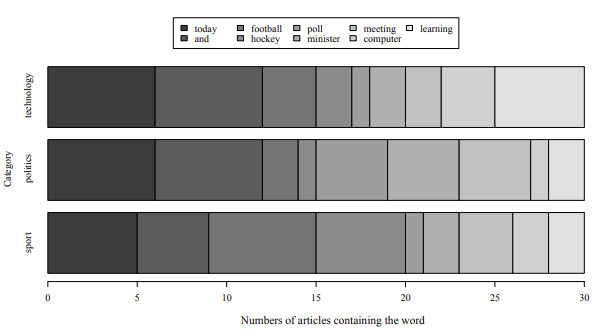
\includegraphics[width=0.6\textwidth]{chapter/chapter14/figure14_5.png}
\captionsetup{labelformat=empty}
\caption{\textbf{Figure 14.5:} Visualization of term distribution across classes.}
\label{fig14.5}
\end{center}
\end{figure}

\begin{verbatim}
    print(paste("Class: ", c))
    # we want only attributes with the average frequency for
    # a class higher than the average for all classes)
    print(sort((chi[c,tab[,c ] > avg_freq]), decreasing=TRUE))
}
\end{verbatim}

The output of the statements follows:\\[0pt]
\begin{verbatim}
[1] "Values of Information gain:"
       attr_importance
today      0.00450826
and        0.01791164
football   0.06239830
hockey     0.07370431
poll       0.05934322
minister   0.02197633
meeting    0.01610484
computer   0.02161919
learning   0.04621363

[1] "Three best attributes:"
[1] "hockey"  "football" "poll"
[1] "50% best attributes:"
[1] "hockey"  "football" "poll"     "learning"


[1] "The values of Chi square for attributes and classes:"
[1] "Class: sport"
hockey football
4.176136 3.516746
[1] "Class: politics"
poll minister meeting and today
3.7500000 1.3636364 0.7142857 0.2678571 0.0678733
[1] "Class: technology"
learning computer and today
2.8571429 0.9375000 0.2678571 0.0678733
\end{verbatim}
